%Manual de Usuario
%Programa de cómputo didáctico
%"Análisis Financiero"
%Ricardo Quezada Figueroa
%Administración financiera
%ESCOM - IPN

\documentclass[oneside,12pt]{article}

%Bibliotecas
\usepackage[spanish,mexico]{babel}                  %Documento en español
\usepackage[utf8]{inputenc}                         %Codificación en utf8
\usepackage[sfdefault]{ClearSans}                   %Fuente sin serifa
\usepackage[letterpaper, headheight=1.0in,
            textwidth=6.5in, inner=1.0in,
			outer=1.0in, bottom=1.0in]
            {geometry}                              %Margenes del documento
\usepackage{graphicx}                               %Manejo de imágenes
\usepackage{float}                                  %Portada
\usepackage{fancyhdr}                               %Encabezado y pie de página
\usepackage{xcolor}                                 %Gestión de colores
\usepackage[]{hyperref}                             %Opciones de pdf producto

%Créditos
\title{Manual de usuario}
\author{Laura Natalia Borbolla Palacios \\
        David Vega Ramírez \\
        Ricardo Quezada Figueroa}

%Encabezado y Pie
\pagestyle{fancy}
\fancyhf{}
\chead{Manual de usuario}
\rfoot{Página \thepage}
\lfoot{Programa de cómputo didáctico ``Análisis Financiero''}
\renewcommand{\headrulewidth}{1pt}
\renewcommand{\footrulewidth}{1pt}

%Configuración de pdf
\hypersetup{
    pdftitle={Manual de usuario},
    pdfauthor={Ricardo Quezada Figueroa},
    pdfsubject={Programa de cómputo didáctico Análisis Financiero},
    bookmarksnumbered=false,
    bookmarksopen=true,
    bookmarksopenlevel=3,
    pdfstartview=Fit,
    pdfpagemode=UseOutlines,
    pdfpagelayout=TwoPageRight,
    colorlinks,
    linkcolor={black!255!black},
    citecolor={black!50!black},
    urlcolor={black!80!black}
}

\begin{document}

    \begin{titlepage}
		\begin{center}
			\vspace*{2.5in}
			\rule{170mm}{0.1mm}\\
			\vspace*{0.2in}
			\begin{Large}
				\textbf{Manual de usuario} \\                   %Título
                \vspace*{0.2in}
                Programa de cómputo didáctico ``Análisis financiero'' basado en razónes financieras\\
			\end{Large}
			\vspace*{0.2in}
			\rule{170mm}{0.1mm}\\
			\begin{large}
				\vspace*{0.8in}
				Josefina Hernández Jaime\\                      %Autor(s)
                \vspace*{0.2in}
				Eduardo Rodríguez Flores\\
				\vspace*{0.2in}
				Yasmín Ivette Jiménez Galán\\
			\end{large}
			\begin{large}
				\vspace*{0.8in}
				Ciudad de México, 21 de Mayo de 2016\\          %Fecha
			\end{large}
		\end{center}
	\end{titlepage}

    \tableofcontents
    \newpage

    \section{Interfaces}
    \hypertarget{IU01}{\subsection{IU01 Página de inicio}}


    \subsubsection{Pantalla de bienvenida}

    Primera sección de la pantalla de inicio.
    Se encuentra el título del sistema, los nombres de los autores y la barra de navegación.

    \begin{figure}[H]
		\begin{center}
			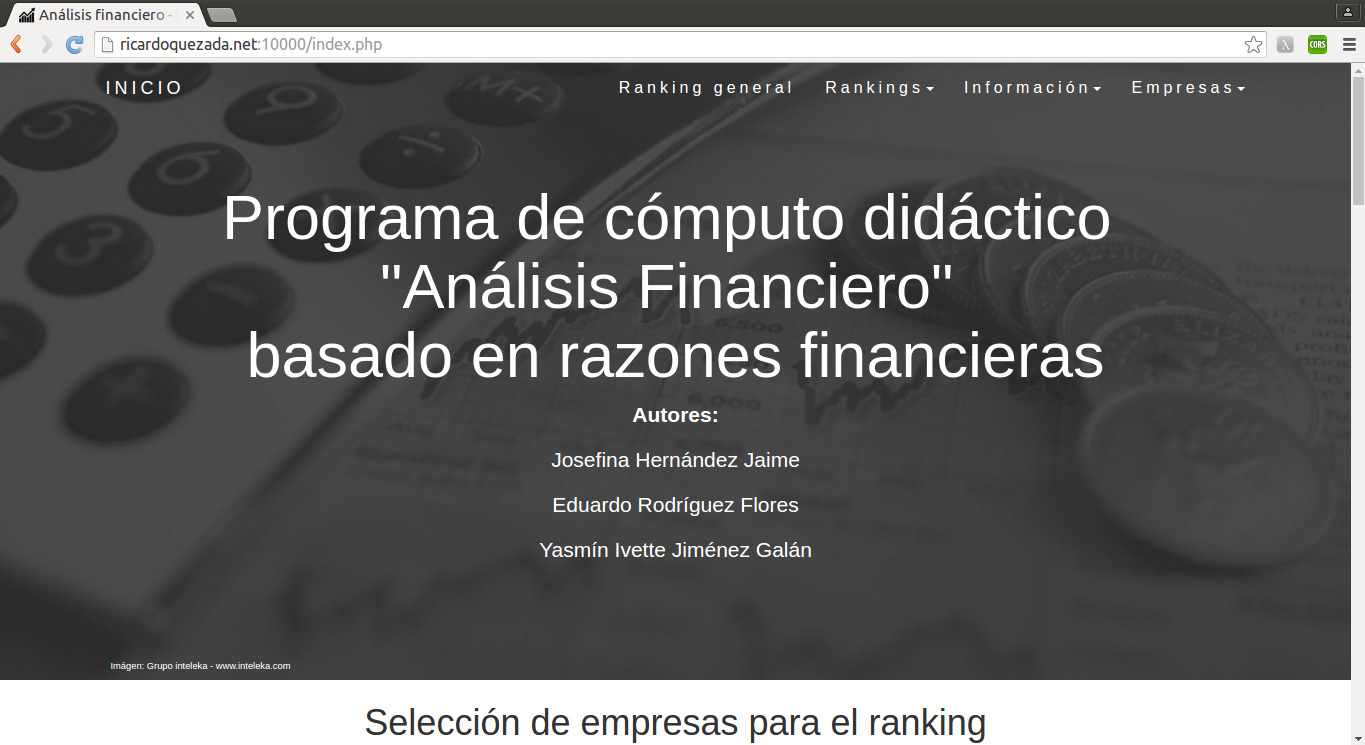
\includegraphics[scale=0.3]{pantallas/Index1}
			\caption{IU01/01 - Pantalla de bienvenida}
		\end{center}
	\end{figure}


    \subsubsection{Pantalla de selección de empresas}

    Para efectuar un análisis, desplácese hacia abajo para ver las empresas listadas.
    Incluya una empresa al análisis presionando sobre su el cuadro de selección a la izquierda de su nombre;
    en él aparecerá una marca, indicando que se considerará en el análisis,
    para eliminar una empresa seleccionada del análisis,
    presionar nuevamente sobre el cuadro a la izquierda,
    la marca desaparecerá.
    ``Seleccionar todo'' marca todos los cuadros y ``Limpiar'' limpia la selección.

    \begin{figure}[H]
		\begin{center}
			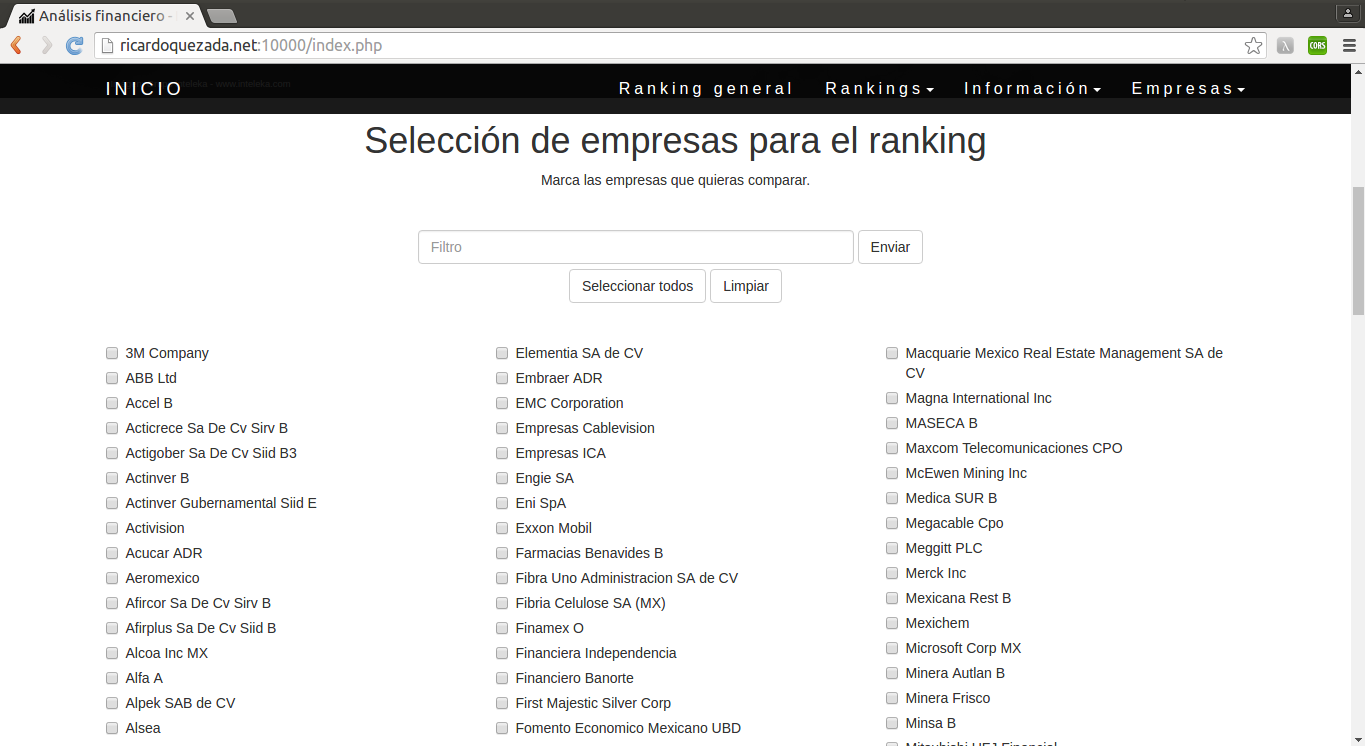
\includegraphics[scale=0.3]{pantallas/Index2}
			\caption{IU01/02 - Pantalla de selección de empresas}
		\end{center}
	\end{figure}


    \subsubsection{Funcionalidad de filtro}

    Introduzca en la barra de búsqueda el nombre de una empresa para encontrarla rápidamente,
    las opciones se reducirán a medida que escribe;
    marque la casilla a su izquierda para agregarla al análisis.

    \begin{figure}[H]
		\begin{center}
			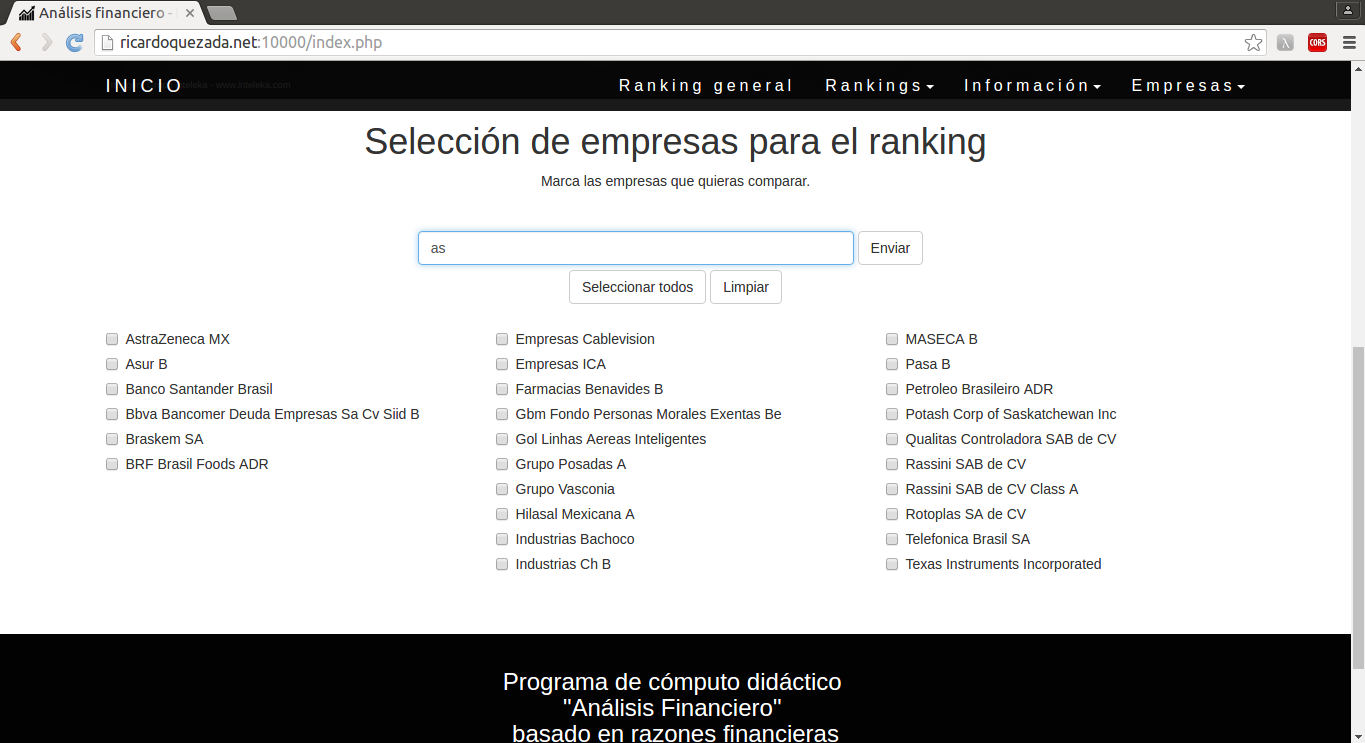
\includegraphics[scale=0.3]{pantallas/Index3}
			\caption{IU01/03 - Funcionalidad de filtro}
		\end{center}
	\end{figure}


    \subsubsection{Pantalla de envío}

    Cuando ya se han seleccionado todas las empresas a considerar,
    presione el botón ``Enviar''.
    La página comenzará a obtener la información.

    Una vez obtenida la información, se redireccióna a la página
    de ranking general.

    \begin{figure}[H]
		\begin{center}
			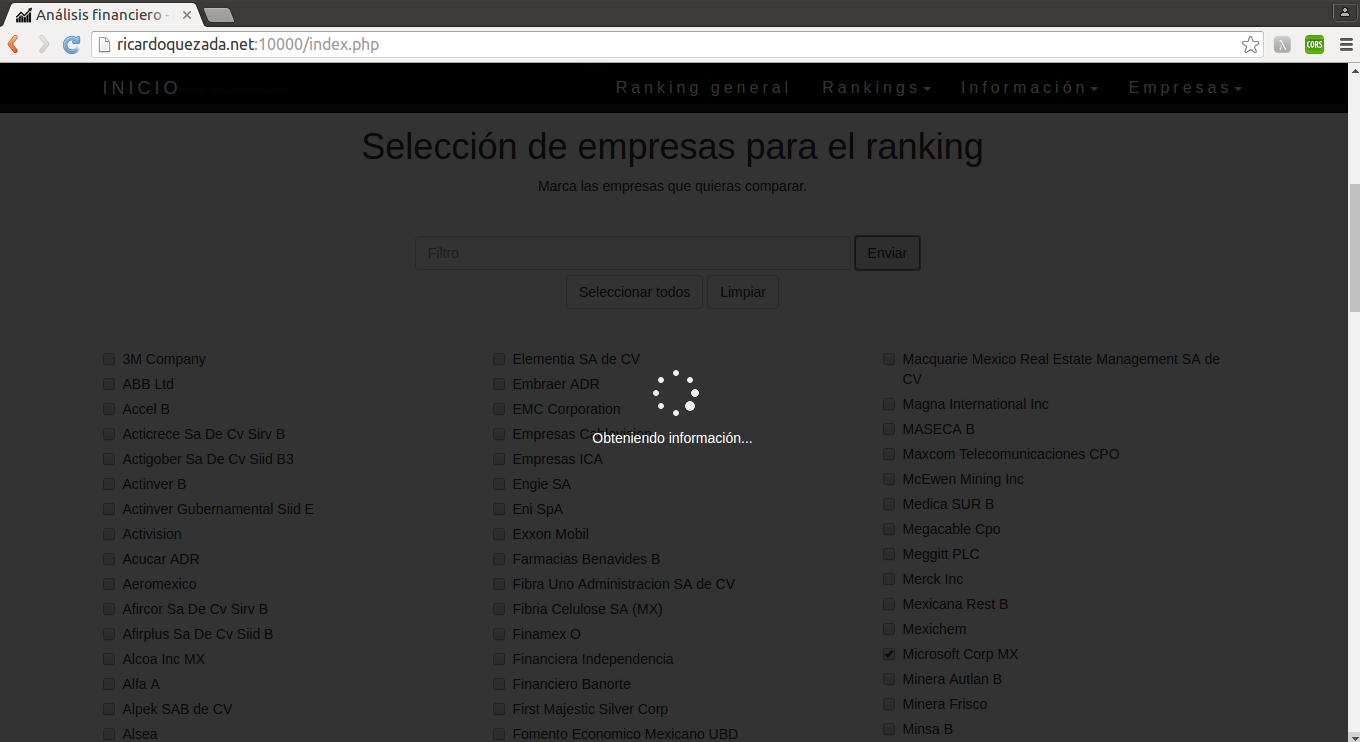
\includegraphics[scale=0.3]{pantallas/Index4}
			\caption{IU01/04 - Funcionalidad de filtro}
		\end{center}
	\end{figure}

    \newpage
    \hypertarget{IU02}{\subsection{IU02 Página de ranking general}}


    \subsubsection{Pantalla de ranking}

    Después de obtener la información se mostrará el ranking general,
    ordenando a las empresas, de manera descendente, por el puntaje general obtenido.
    Este puntaje da prioridad tanto a la rentabilidad
    como a la liquidez de cada empresa sobre el endeudamiento y la rotación.

    \begin{figure}[H]
        \begin{center}
            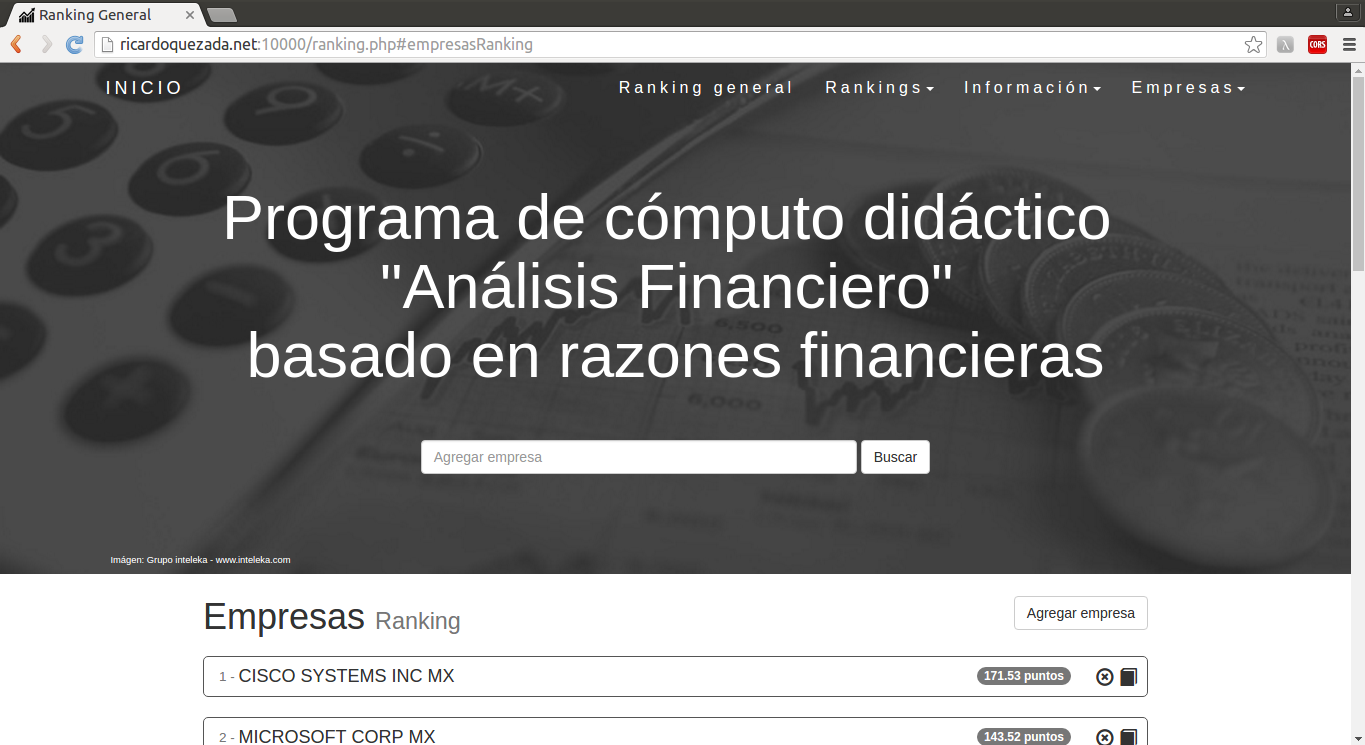
\includegraphics[scale=0.3]{pantallas/Ranking1}
            \caption{IU02/01 - Pantalla de ranking y búsqueda}
        \end{center}
    \end{figure}


    \subsubsection{Funcionalidades de ranking}

    Presione el botón con una cruz al centro para eliminar a esa empresa del análisis.
    Para obtener más información sobre una empresa, presione el ícono del libro correspondiente.

    Presione ``Agregar empresa'' para incluir en el análisis una empresa nueva, ajena al programa.
    Esta última opción abre en una nueva pestaña la página de agregar empresa.

    \begin{figure}[H]
        \begin{center}
            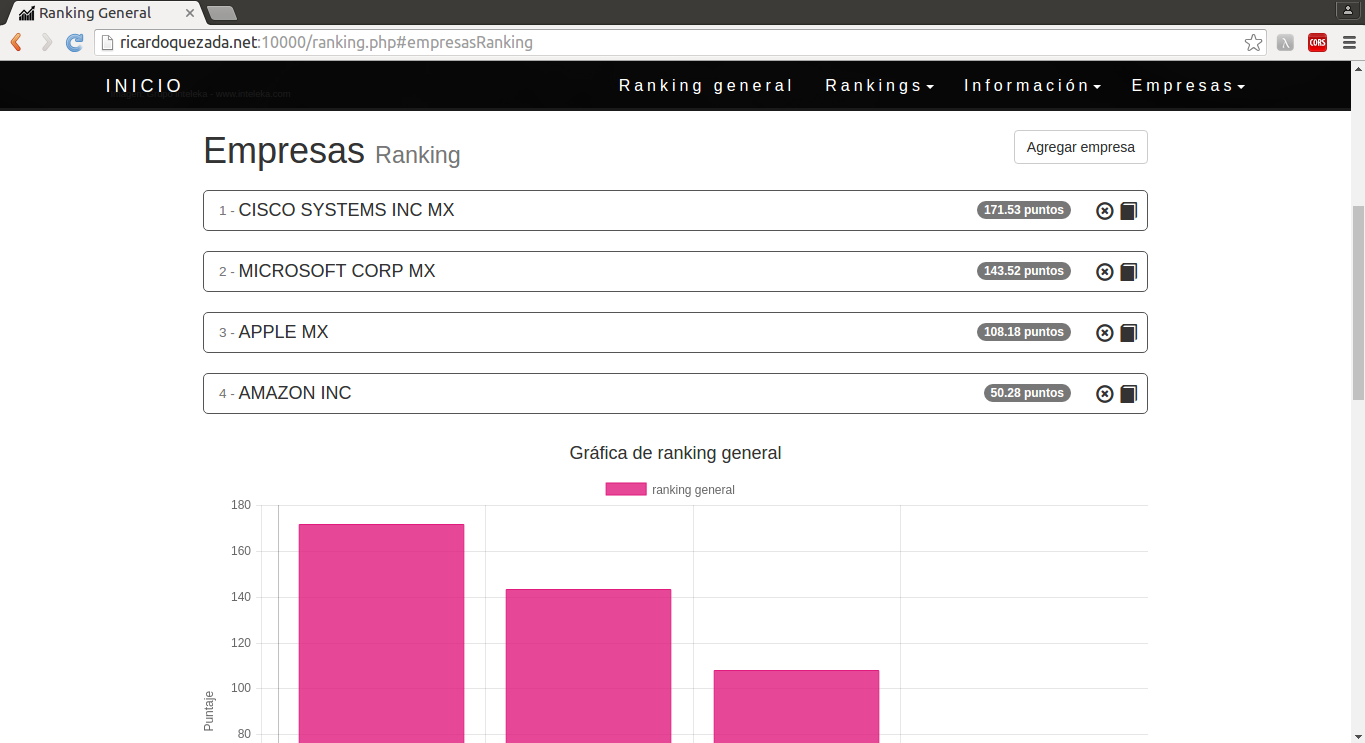
\includegraphics[scale=0.3]{pantallas/Ranking2}
            \caption{IU02/02 - Funcionalidades de ranking}
        \end{center}
    \end{figure}

    Introduzca el nombre de una nueva empresa en la barra de búsqueda para contemplarla en el análisis,
    las opciones irán mostrándose a medida que se escribe; para incluirla presione sobre su nombre 
    y despues sobre ``buscar''.

    \begin{figure}[H]
        \begin{center}
            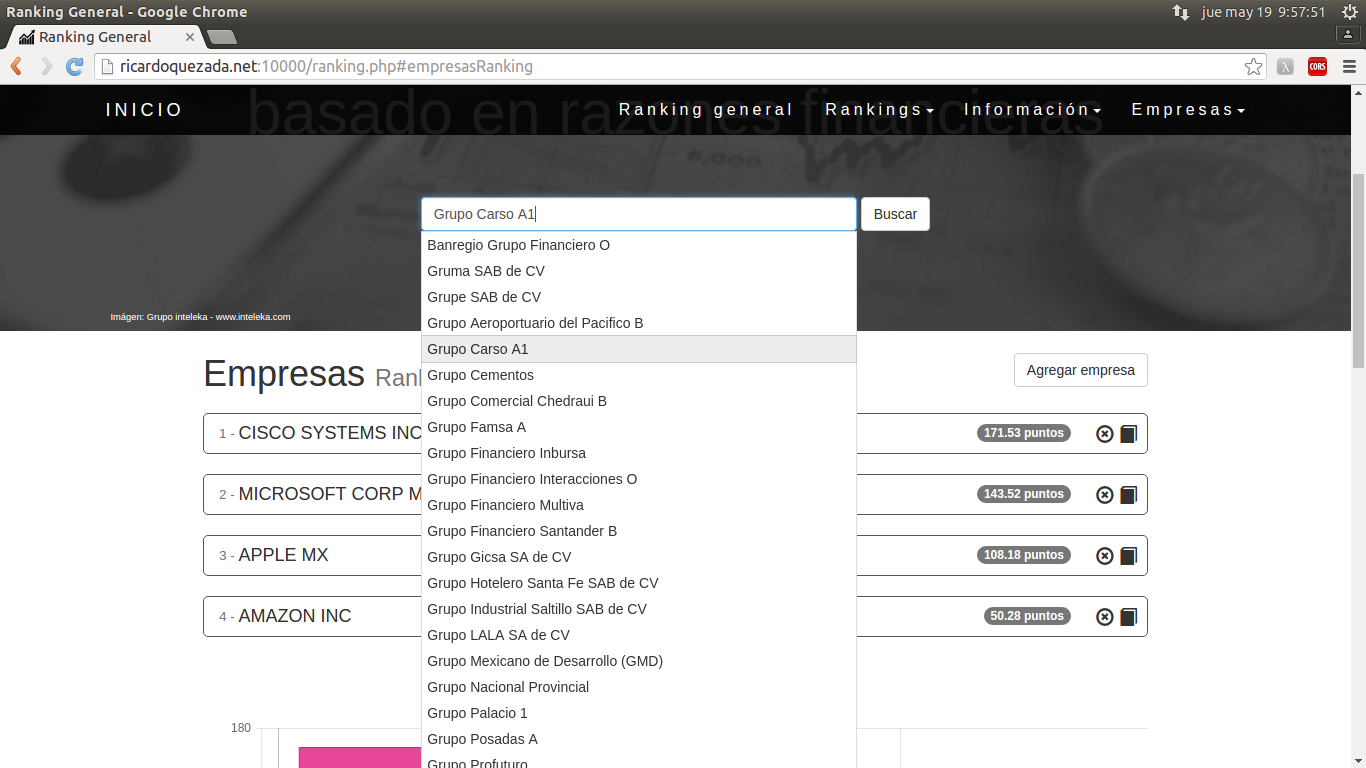
\includegraphics[scale=0.3]{pantallas/Ranking3}
            \caption{IU02/03 - Búsqueda de empresa}
        \end{center}
    \end{figure}


    \subsubsection{Funcionalidades de gráficas}

    Desplácese hacia abajo para ver una gráfica de barras el puntaje general obtenido por cada empresa.
    Pase el cursor sobre una barra para ver los puntos obtenidos y el nombre de la empresa correspondiente.

    \begin{figure}[H]
        \begin{center}
            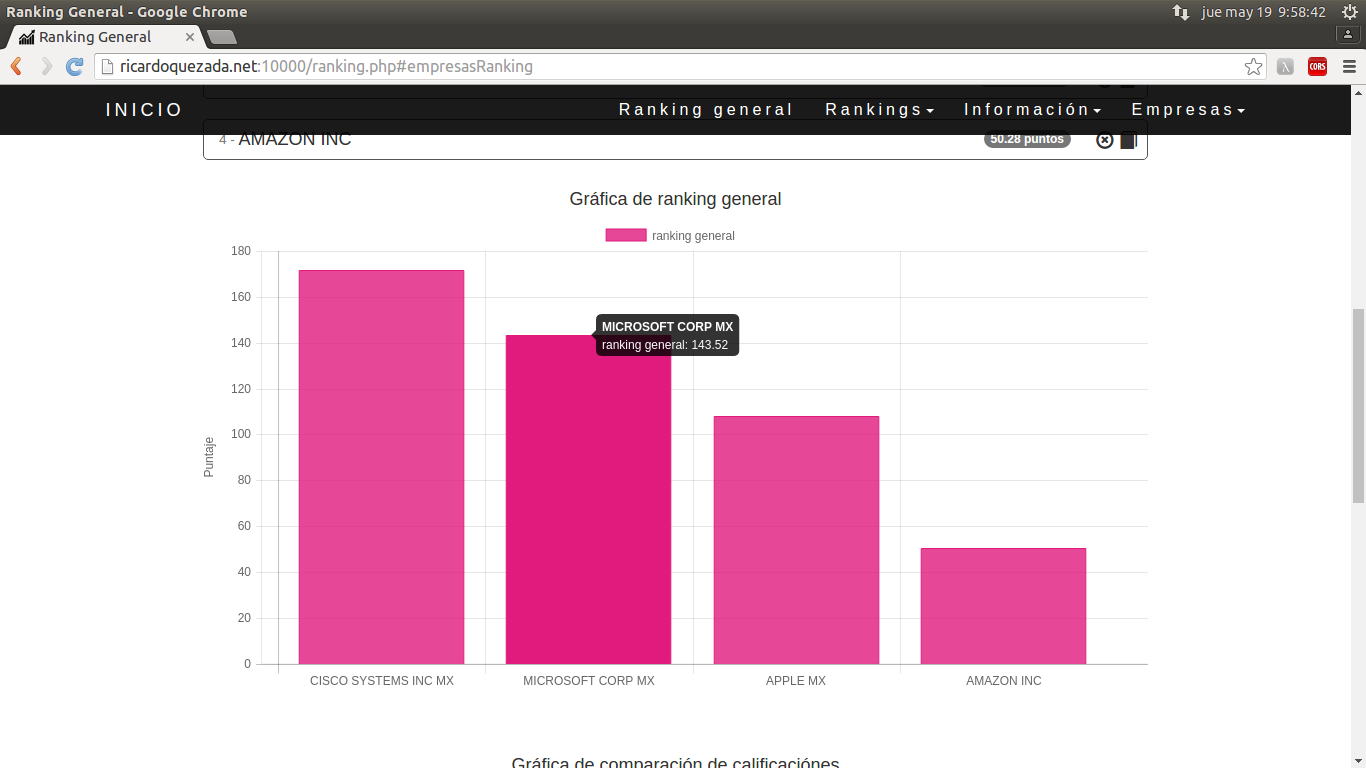
\includegraphics[scale=0.3]{pantallas/Ranking4}
            \caption{IU02/04 - Gráfica de barras de ranking general}
        \end{center}
    \end{figure}

    Desplácese más abajo para encontrar una gráfica de radar que compara el puntaje obtenido
    por cada empresa en los índices de rentabilidad, liquidez, rotaciones y endeudamiento.
    Entre mayor sea el área, mayor será su puntaje general.

    Presione sobre el nombre de una empresa para quitarla de la gráfica y observar a las otras
    con mayor detenimiento, la escala se reajustará automáticamente para las que queden
    seleccionadas y el nombre se verá tachado. Pulse sobre el nombre tachado
    para mostrarla nuevamente en la gráfica.

    Pase el cursor sobre un punto par observar el puntaje obtenido
    por esa empresa en el eje en que se encuatre.


    \begin{figure}[H]
        \begin{center}
            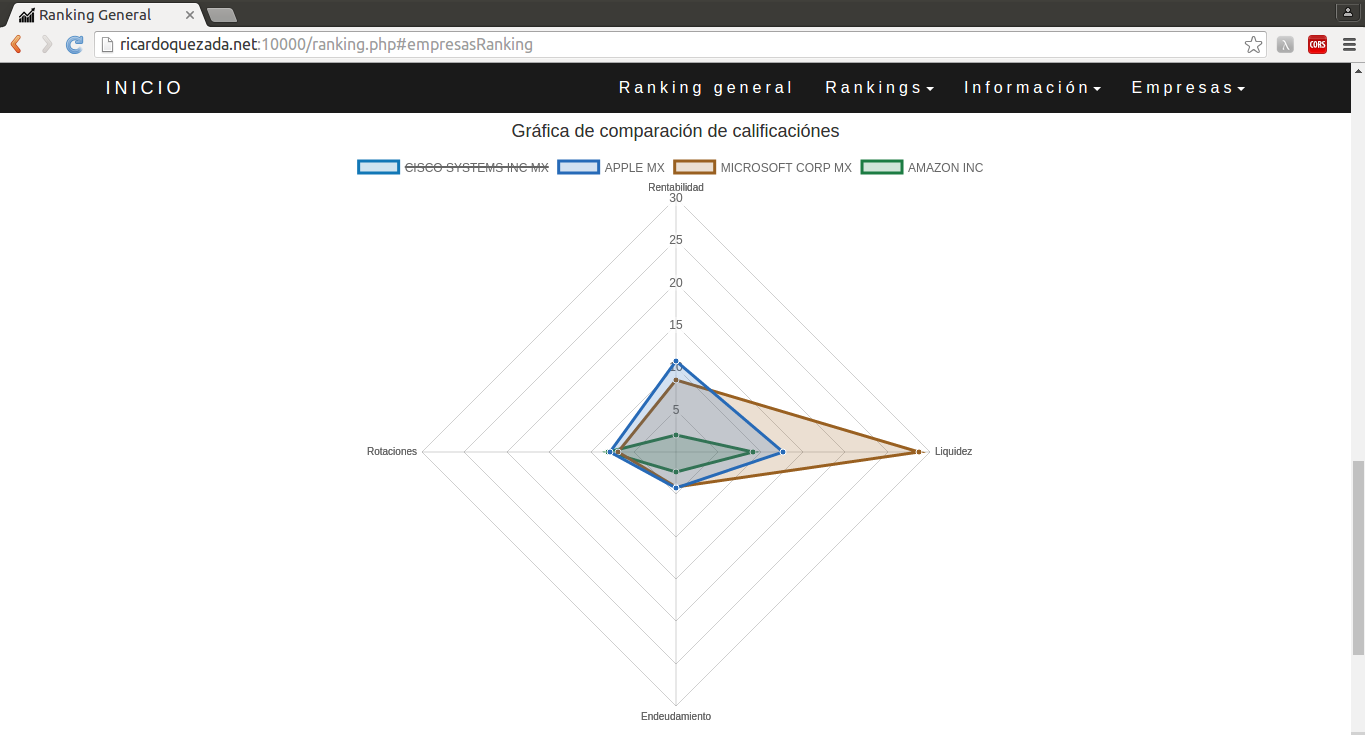
\includegraphics[scale=0.3]{pantallas/Ranking5}
            \caption{IU02/05 - Gráfica de radar de ranking general}
        \end{center}
    \end{figure}

    \newpage
    \hypertarget{IU03}{\subsection{IU03 Página de empresa}}


    \subsubsection{Pantalla de datos}

    Después de presionar el botón para ver más información sobre una empresa,
    se abrirá una nueva pestaña en el navegador con sus datos.
    Primero se muestran los datos financieros (activos, pasivos y capital contable)
    con los que se han calculado las razones. Presione ``Editar registro''
    para modificar la información de la empresa.

    \begin{figure}[H]
        \begin{center}
            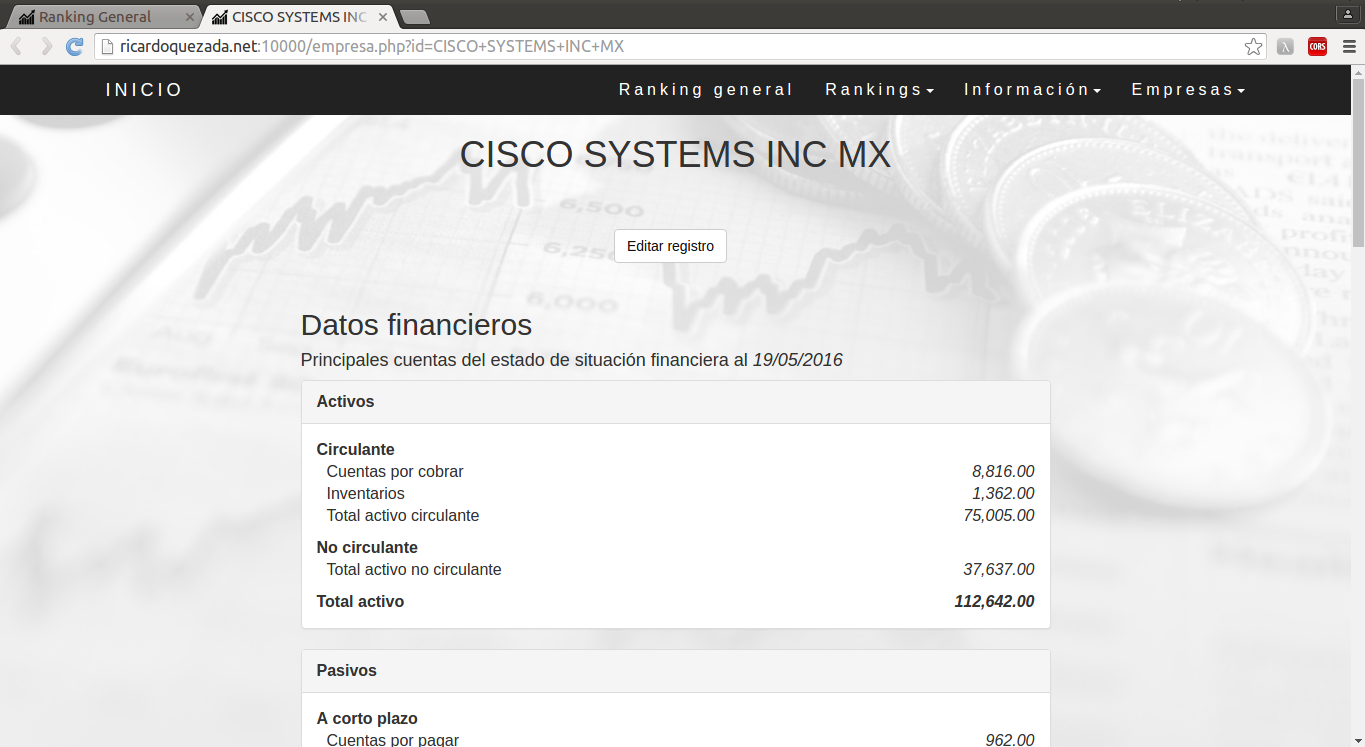
\includegraphics[scale=0.3]{pantallas/Empresa1}
            \caption{IU03/01 - Pantalla de datos}
        \end{center}
    \end{figure}


    \subsubsection{Pantalla de índices}

    Más abajo se encuentran las razones simples para dicha empresa,
    separados por índices. Cada índice tiene dos enlaces,
    uno para obtener información sobre ese índice y las razones que lo componen 
    y otro para ir al ranking de ese índice.

    \begin{figure}[H]
        \begin{center}
            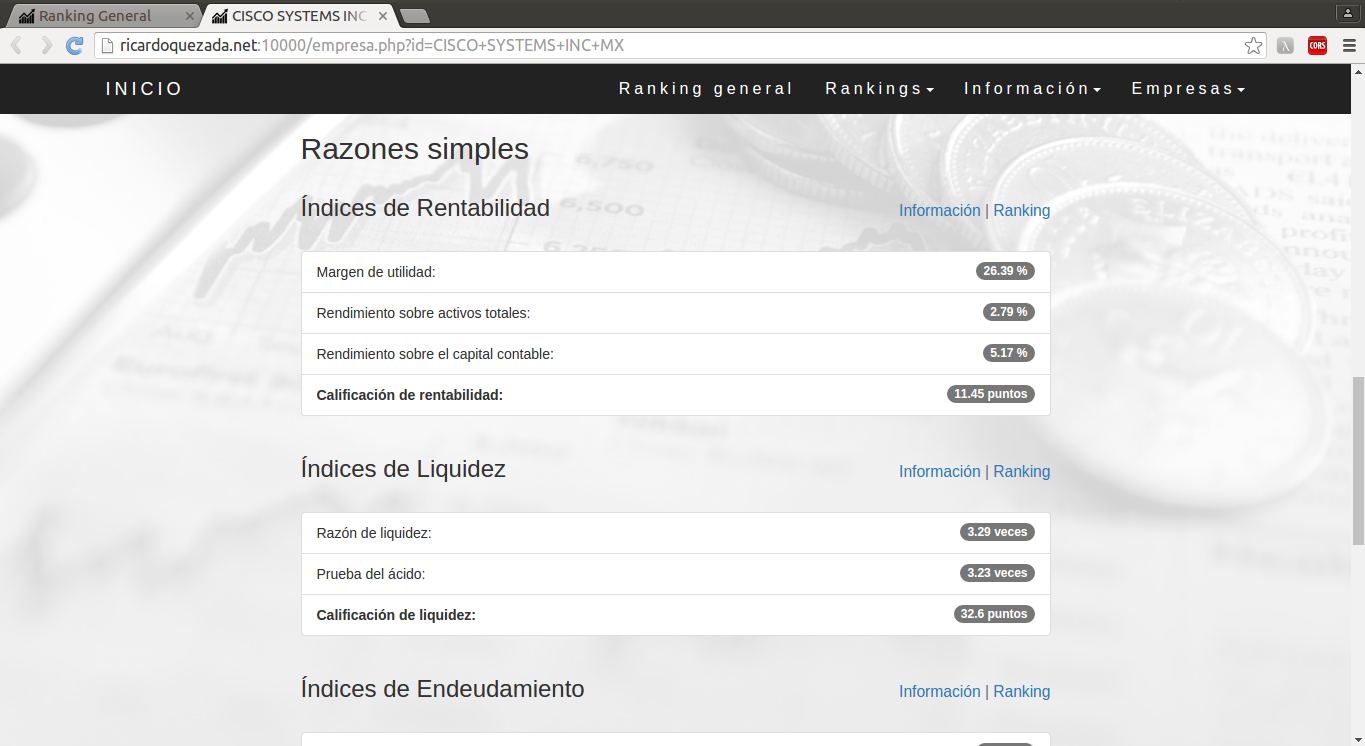
\includegraphics[scale=0.3]{pantallas/Empresa2}
            \caption{IU03/01 - Pantalla de índices}
        \end{center}
    \end{figure}

    \newpage
    \hypertarget{IU04}{\subsection{IU04 Página de edición de registros}}

    Al editar una empresa, los datos actuales se mostrarán sus cambios,
    modifique los campos deseados y presione ``Enviar'' para guardarlos.
    Pulse ``Borrar registro'' para eliminar a la empresa del programa.

    \begin{figure}[H]
        \begin{center}
            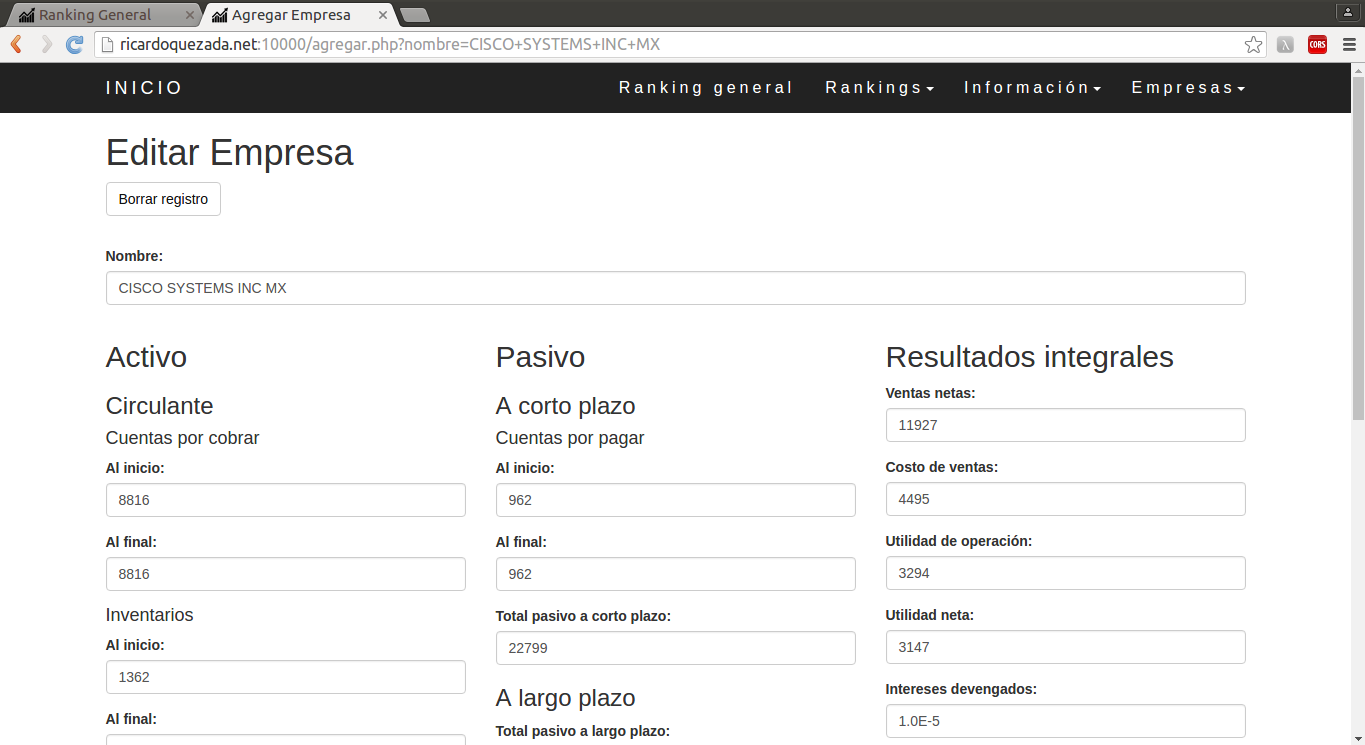
\includegraphics[scale=0.3]{pantallas/Editar1}
            \caption{IU04/01 - Formulario de edición}
        \end{center}
    \end{figure}

    \newpage
    \hypertarget{IU05}{\subsection{IU05 Página de adición de empresas}}

    Ingrese la información de la nueva empresa, al terminar presione ``Enviar''.
    Sus razones serán calculadas y será incluida en el análisis actual.

    Ya que esta empresa no será guardada,
    no será posible considerarla al hacer un análisis nuevo.

    \begin{figure}[H]
        \begin{center}
            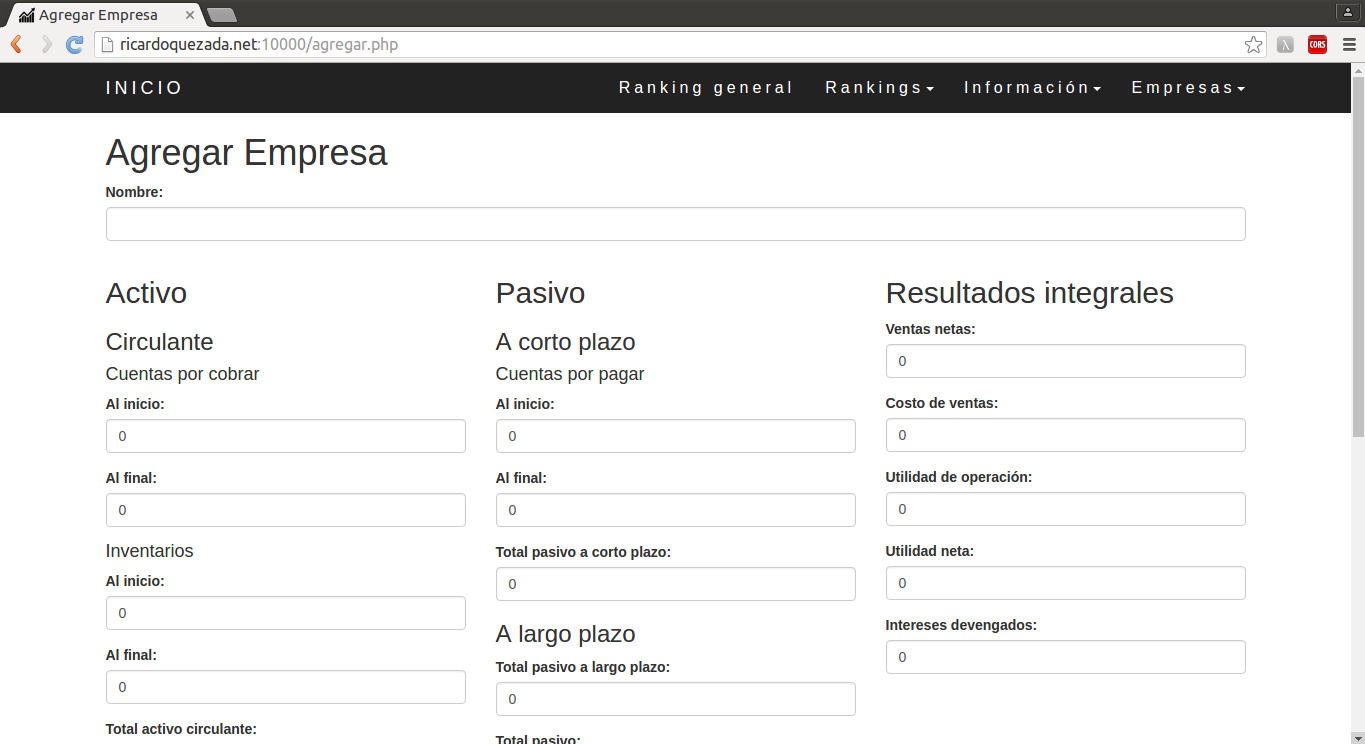
\includegraphics[scale=0.3]{pantallas/Agregar1}
            \caption{IU05/01 - Formulario de adición}
        \end{center}
    \end{figure}

    \newpage
    \hypertarget{IU06}{\subsection{IU06 Páginas de rankings por grupo}}

    Presionar en la barra de navegación ``Rankings'', después el índice deseado
    para ir a su escalafón. Las empresas aparecen ordenadas descendentemente
    por el puntaje obtenido en ese índice, después una gráfica de barras que muestra el
    puntaje total obtenido en ese índice por empresa.

    Más abajo aparecen rankings de cada una de las razónes que componen a ese índice.
    De cada ranking se muestra una tabla y una gráfica.

    Presionar el enlace ``Información'' para obtener información sobre el índice.

    \begin{figure}[H]
        \begin{center}
            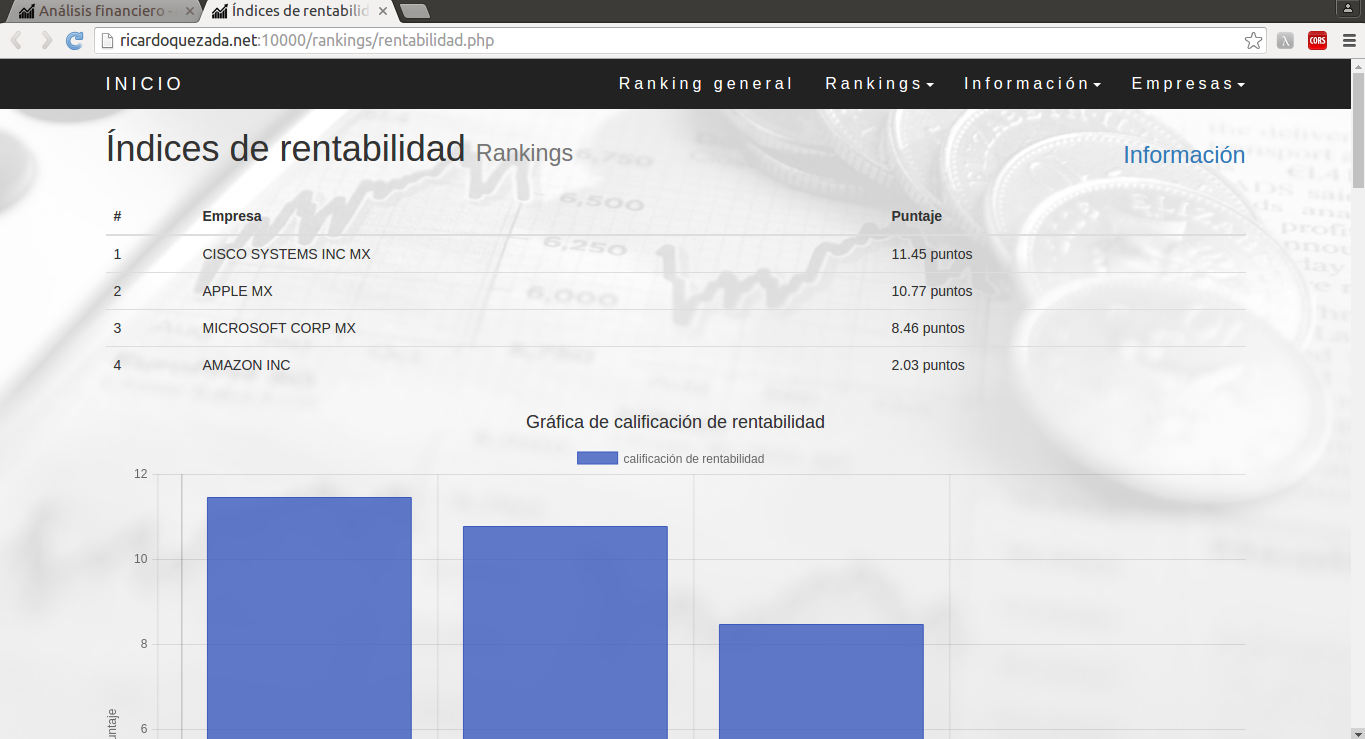
\includegraphics[scale=0.3]{pantallas/Rankings1}
            \caption{IU06/01 - Ranking por grupo}
        \end{center}
    \end{figure}

    \newpage
    \hypertarget{IU07}{\subsection{IU07 Páginas de informacion de razónes}}

    Después de presionar el enlace a información, se abre una nueva pestaña
    mostrando cada una de las razones simples que están contenidas en este índice
    (su interpretación, fórmula para obtenerla y una calculadora).

    \begin{figure}[H]
        \begin{center}
            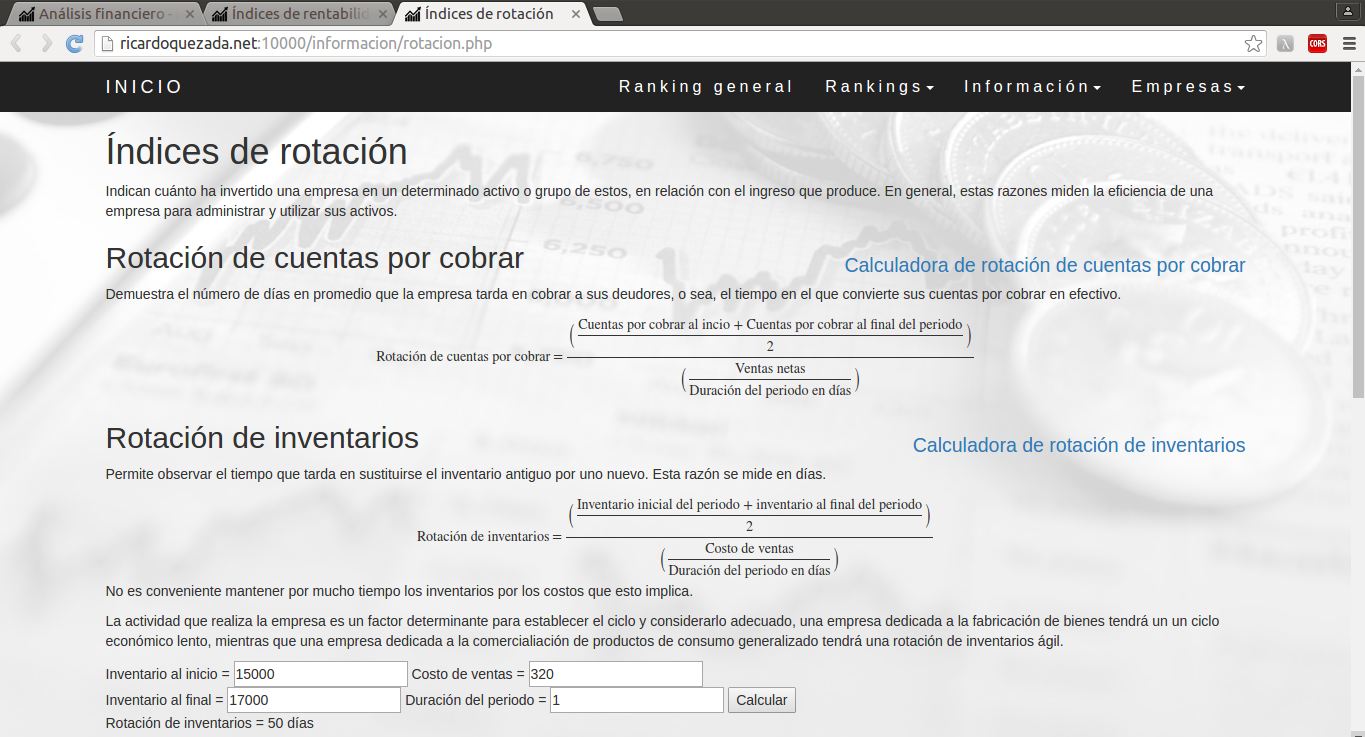
\includegraphics[scale=0.3]{pantallas/Info1}
            \caption{IU07/01 - Información de razónes}
        \end{center}
    \end{figure}

    \newpage
    \hypertarget{IU08}{\subsection{IU08 Barra de navegación}}

    Presionar en “Ranking general” para dirigirse a la página del ranking general del análisis.
    Presionar en la barra de navegación “Rankings” para ver una lista desplegable de los rankings
    por índice que son calculados para el análisis.
    Presione en cualquiera de los índices para dirigirse a la página del ranking de ese índice.

    \begin{figure}[H]
        \begin{center}
            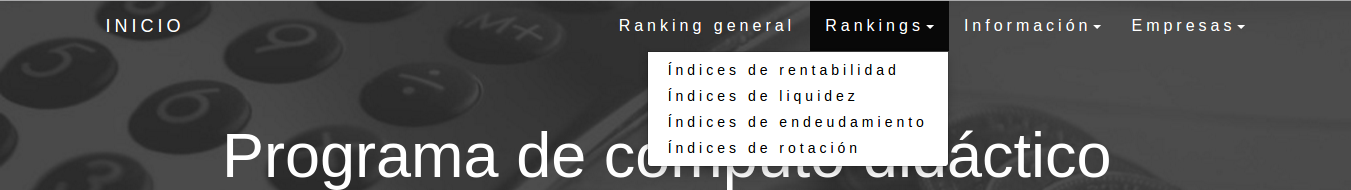
\includegraphics[scale=0.3]{pantallas/Navegacion1}
            \caption{IU08/01 - Navegación 1}
        \end{center}
    \end{figure}


    Presionar en la barra de navegación “Información” para ver una lista desplegable
    de los índices de razones simples que calculados para el análisis.
    Presione en cualquiera de para dirigirse a la página de información de ese índice.

    \begin{figure}[H]
        \begin{center}
            
\includegraphics[scale=0.3]{pantallas/Navegacion2}
            \caption{IU08/01 - Navegación 2}
        \end{center}
    \end{figure}


    Presionar en la barra de navegación “Empresas” para ver una lista desplegable
    de las empresas consideradas para este análisis. Presione en cualquiera de
    ellas para dirigirse a la página de información de esa empresa.

    \begin{figure}[H]
        \begin{center}
            
\includegraphics[scale=0.3]{pantallas/Navegacion3}
            \caption{IU08/01 - Navegación 3}
        \end{center}
    \end{figure}



\end{document}
